\section{A Bomba}
A bomba participa dos dois sistemas referênciados acima: sistema de propulsão e limpeza. O processo de aspiração da piscina feito pelo robô será uma das principais tarefas executadas pela bomba de sucção, bem como também o processo de movimentação do robô embaixo d’água. Para isso, é importante que a bomba seja  forte o suficiente para sugar e gerar movimentação por meio do fluxo de saída da bomba. A sucção será conectada diretamente ao reservatório onde acontecerá a filtragem da água. É importante ressaltar que as únicas funções da bomba neste projeto são apenas filtrar e movimentar o robô através do empuxo gerado.

A análise do dimensionamento adequado para a bomba será feito a partir de sua vazão nominal. Para isto, tem-se por especificações primárias bombas que ofereçam vazões altas e que trabalhem em uma profundidade máxima de 3 metros.

\subsection{O Dimensionamento}
Para que pudesse definir qual bomba adquirir foi necessário realizar o dimensionamento da mesma, afim de que a bomba pudesse realizar a sucção da água e a  propulsão do robô abaixo d’água. Para isso, é necessário utilizar métodos que descrevem os cálculos que regem o movimento. Segundo
\citeonline{ise2000}, quando um veículo submersível se movimenta com velocidade constante,
a propulsão gerada pelos propulsores se iguala à força de arrasto produzida. A
força de arrasto será obtida a partir da soma da força de arrasto devido a
movimentação do veículo mais a força de arrasto devido o cabo de alimentação.

\begin{equation} \label{eq:force-propulsion}
  Fp = Fa = Fv + Fc = \frac{1}{2}\rho V^{2}_{v}Cd_{v} + \frac{1}{2}\rho V^{2}_{c}Cd_{c}
\end{equation}

Onde $Fp$ e $Fa$ referem-se à força de propulsiva e força de arrasto total
respectivamente; $Fv$ e $Fc$ são as forças de arrasto devido ao veiculo e ao cabo de
alimentação; $\rho$ é a densidade do fluido, $V_{v}$ e $V_{c}$ velocidades do
veículo e do cabo e por fim, $Cd_{v}$ e $Cd_{c}$ representam os coeficientes
de arrasto.
\par
A potência necessária para a bomba pode ser obtida em função da força propulsiva
e da velocidade do veiculo.
\begin{equation} \label{eq:force-propulsiva}
  P = Fp\frac{d}{t}
\end{equation}
Onde $d$ é a distancia percorrida, $t$ o tempo e $P$ a potência desejada.
\par
Os coeficientes de arrasto são medidos experimentalmente, para fluidos como
ar podem ser encontrados tabelados em função da velocidade do veiculo em relação
à velocidade do som nas condições do ambiente em questão (número de \textit{Mach}), uma
vez que este pode sofrer alterações devido a temperatura envolvida, meio de
propagação etc. Quando o veículo estudado se movimento em fluido líquido como a
água por exemplo, o coeficiente de arrasto deve ser medido em função do número
de Reynolds \cite{eng2008}, que por sua vez é calculado pela equação abaixo.

\begin{equation} \label{eq:reynolds}
  Re = \frac{VD}{\upsilon}
\end{equation}

Onde $V$ equivale a velocidade do veículo, $D$ o diâmetro e $\upsilon$ a viscosidade
cinemática do fluido.
\par
\begin{figure}[h]
  \centering
  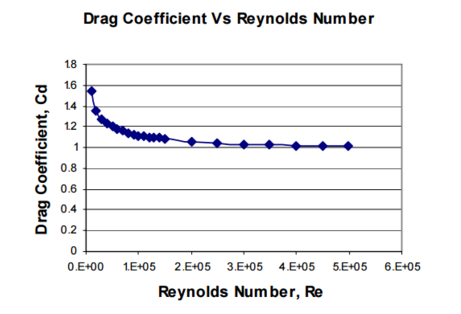
\includegraphics[width=0.9\textwidth]{figures/graphic-reynolds.png}
  \caption{Coeficiente de arrasto em função do número de Reynolds \cite{eng2008}}
  \label{fig:graphic-reynolds}
\end{figure}
\FloatBarrier
\par
Aplicando-se a Equação \ref{eq:force-propulsion} para o objeto deste trabalho, temos:
\begin{displaymath}
  Fp = Fa = Fv + Fc = \frac{1}{2}\rho V^{2}_{v}Cd_{v} + \frac{1}{2}\rho V^{2}_{c}Cd_{c}
\end{displaymath}
\begin{displaymath}
  \rho = 1000 kg/m^{3}
\end{displaymath}

Substituindo os valores de $\rho$, assumindo uma velocidade de operação de 0,14 m por segundo e $Cdv = 1$ e desprezando o arrasto gerado pelo cabo (a força de arrasto do cabo é compensada por se considerar o pior caso em que o arrasto é igual a 1). Temos que $Fa = 70N$.

Com os dados de tempo, velocidade e força necessaria para a impulsão do robo chega-se a vazão necessaria do sistema de propulsão. A vazão necessaria para a propulsão proposta é de 5000 litros por hora, pouco mais de 1300 galoões por hora. Boa parte dessa propulsao virá da bomba principal descrita logo mais a seguir, o restante será compensado com o uso de um motor acoplado ao duto de saída como explicado anteriormente.

\subsection{A Escolha da Bomba}
O modelo proposto será uma bomba do tipo \textsf{Bilge}, com as seguintes características:
\begin{itemize}
\item Peso: aproximadamente 3 kg
\item Modelo: 1100 GPH - com Tensão de trabalho 12 V DC - Amperagem de 3,3;
\item Formato: Cilíndrico alterável;
\item Área de operação entorno de até 3,7 metros;
\end{itemize}

A bomba comercial a ser utilizada esta apresentada abaixo:
\par
\begin{figure}[h]
  \centering
  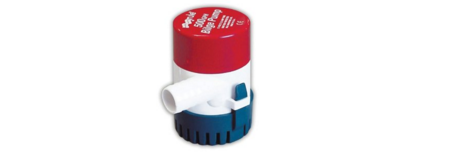
\includegraphics[width=0.9\textwidth]{figures/waterbomb.png}
  \caption{Bilge Pump}
  \label{fig:waterbomb}
\end{figure}
\FloatBarrier
\par
